\begin{theorem} (1907г. Ф. Рисс, Фишер)
	Пусть $H$ --- сепарабельное гильбертово пространство, $e = \{e_n\}_{n = 1}^\infty \subseteq H$ --- ортонормированная система. Тогда следующие условия равносильны:
	\begin{enumerate}
		\item $e$ --- базис Шаудера
		
		\item $e$ --- полная система
		
		\item $e^\bot = \{0\}$
		
		\item Выполнено равенство Парсеваля: $\forall x \in H\ \|x\|^2 = \sum_{i = 1}^\infty |(x, e_i)|^2$
	\end{enumerate}
\end{theorem}

\begin{lemma} (Минимальное свойство коэффициентов Фурье)
	Пусть $\{e_n\}_{n = 1}^N \subseteq H$ --- ортонормированная система. Тогда выполнено неравенство:
	\[
	\forall \{\alpha_n\}_{n = 1}^N \subset \R\ \ \no{x - \sum_{n = 1}^N (x, e_n)e_n} \le \no{x - \sum_{n = 1}^N \alpha_n e_n}
	\]
	Иначе говоря, сумма Фурье является наилучшим приближением среди всех других сумм.
\end{lemma}

\begin{proof}
	Во-первых, базовое правило для выведения неравенств состоит в том, что надо работать с квадратом нормы. Во-вторых, мы просто оценим квадрат нормы справа, расписав его в явном виде (а чтобы выделить в равенствах выражение слева, мы вычтем и добавим соответствующие суммы):
	\begin{multline*}
	\no{x - \sum_{n = 1}^N \alpha_n e_n}^2 = \|x\|^2 + \no{\sum_{n = 1}^N \alpha_n e_n}^2 - 2\sum_{n = 1}^N \alpha_n (x, e_n) =
	\\
	\|x\|^2 - \sum_{n = 1}^N |(x, e_n)|^2 + \sum_{n = 1}^N \alpha_n^2 - 2\sum_{n = 1}^N \alpha_n(x, e_n) + \sum_{n = 1}^N |(x, e_n)|^2 =
	\\
	\no{x - \sum_{n = 1}^N (x, e_n)e_n}^2 + \sum_{n = 1}^N (\alpha_n - (x, e_n))^2 \ge \no{x - \sum_{n = 1}^N (x, e_n)e_n}^2
	\end{multline*}
\end{proof}

\begin{center}
	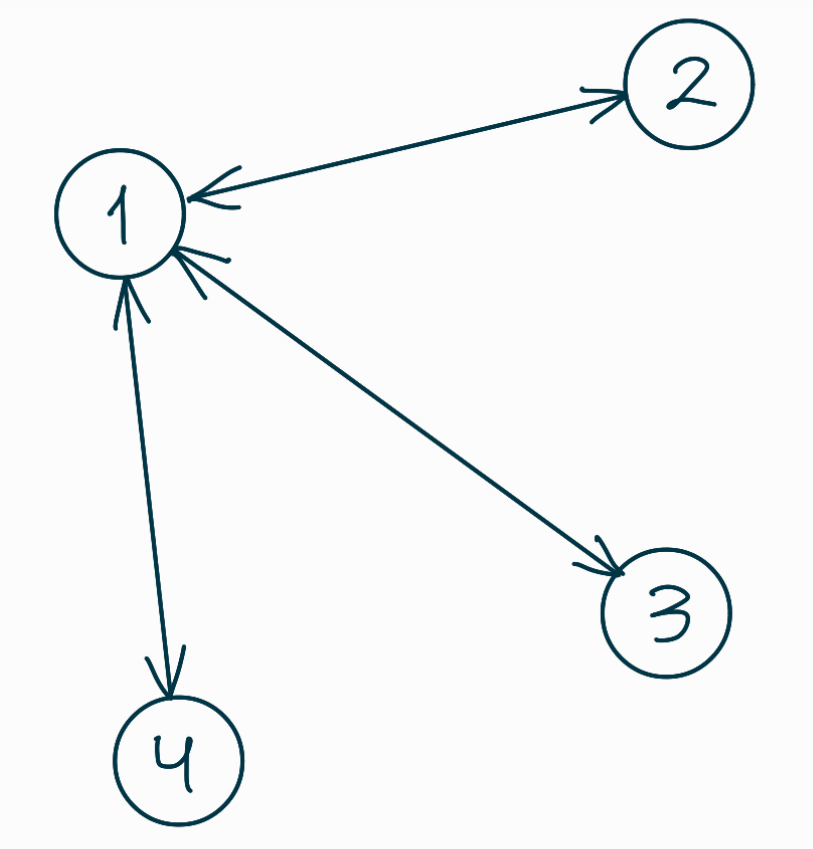
\includegraphics[width=0.25\textwidth]{images/2pic.png}
	\captionof*{figure}{Схема доказательства теоремы Рисса-Фишера}
\end{center}

\begin{proof} (теоремы Рисса-Фишера)
	\begin{itemize}
		\item[$1 \Lra  4$] Воспользуемся равенством Бесселя:
		\[
			\no{x - \sum_{n = 1}^N (x, e_n)e_n}^2 = \|x\|^2 - \sum_{n = 1}^N |(x, e_n)|^2
		\]
		Так как сходимость частичных сумм ряда к $x$ эквивалентна стремлению нормы слева к нулю, то всё доказано автоматически.
		
		\item[$1 \Ra 2$] Тривиально
		
		\item[$1 \La 2$] Для доказательства воспользуемся леммой о минимальном свойстве коэффициентов Фурье. Итак, $e$ --- полная система. Это значит, что любой $x \in H$ можно сколь угодно хорошо приблизить:
		\[
			\forall \eps > 0\ \exists T = \sum_{n = 1}^N \alpha_n e_n\ \no{x - \sum_{n = 1}^N \alpha_n e_n} < \eps
		\]
		Стало быть, в силу минимального свойства сумм Фурье верно следующее:
		\[
			\forall \eps > 0\ \exists N \in \N \such \|S_N(x) - x\| \le \|T - x\| < \eps
		\]
		Отсюда же мы сразу получаем сходимость сумм Фурье:
		\[
			\forall \eps > 0\ \exists N \in \N \such \forall n \ge N\ \ \|S_n(x) - x\| \le \|S_N(x) - x\| < \eps
		\]
	
		\item[$1 \Lra 3$] Пусть $M = \cl [e]$. Тогда, по теореме о проекции $M \oplus M^\bot = H$. Дальше всё просто:
		\begin{itemize}
			\item[$\Ra$] Тривиально, раз $M = H$ сразу.
			
			\item[$\La$] Понятно, что $M^\bot$ требует ортогональности своих элементов к каждому элементу $M$, в частности $e$. Поэтому, если $e^\bot = \{0\}$, то $M^\bot = \{0\}$ и тогда $M = H$.
		\end{itemize}
	\end{itemize}
\end{proof}

\begin{theorem}
	Пусть $H$ --- бесконечномерное сепарабельное гильбертово пространство. Тогда в $H$ существует ортонормированный базис.
\end{theorem}

\begin{note}
	Должно быть очевидно, что, если в $H$ есть не более чем счётный базис, то $H$ --- сепарабельно.
\end{note}

\begin{proof}
	Пусть $X = \{x_n\}_{n = 1}^\infty$ --- это всюду плотное счётное множество в $H$. Так как у нас имеется процесс Грама-Шмидта, то мы можем выделить в $X$ ортонормированный базис. Коль скоро $H = [X]$, то этот базис $X$ будет полным в $H$, а по уже доказанному, стало быть, эта система будет базисом $H$.
\end{proof}

\begin{definition}
	\textit{Изоморфизмом евклидовых пространств $E_1$, $E_2$} называется отображение $\phi \colon E_1 \to E_2$, которое является изоморфизмом линейных пространств и \textit{уважает скалярное произведение}:
	\[
		\forall x, y \in E_1\ \ (x, y)_1 = (\phi(x), \phi(y))_2
	\]
\end{definition}

\begin{theorem}
	Если $H$ --- сепарабельное гильбертово пространство, то $H$ изоморфно пространству $\ell_2(\K)$.
\end{theorem}

\begin{proof}
	В сепарабельном гильбертвом пространстве есть ортонормированный базис $e$. Если рассмотреть $H$ как пространство с евклидовой метрикой, порождённой базисом $e$, то будет тривиальный изоморфизм пространств $H \cong \ell_2(\K)$ (каждому вектору ставим в соответствие его коэффициенты разложения по базису $e$).
\end{proof}

\section{Линейные ограниченные (непрерывные) операторы}

\begin{note}
	Далее обозначения $E_1, E_2$ используются для обозначения линейных нормированных пространств.
\end{note}

\begin{definition}
	Любое отображение $A \colon E_1 \to E_2$ называется \textit{оператором}.
\end{definition}

\begin{reminder}
	По возможности скобки для аргумента опускаются, $Ax := A(x)$.
\end{reminder}

\begin{definition}
	Оператор $A \colon E_1 \to E_2$ называется \textit{линейным}, если выполнено утверждение:
	\[
		\forall \alpha, \beta \in \K, x ,y \in E_1\ \ A(\alpha x + \beta y) = \alpha Ax + \beta Ay
	\]
\end{definition}

\begin{proposition} (не по лектору)
	Если $A$ --- линейный оператор, то $A0 = 0$.
\end{proposition}

\begin{proof}
	Действительно, если $A$ линеен, то верно такое равенство:
	\[
		A0 = A(0 + 0) = A0 + A0 \Ra A0 = 0
	\]
\end{proof}

\begin{definition}
	Оператор $A \colon E_1 \to E_2$ называется \textit{ограниченным}, если образ любого ограниченного множества из $E_1$ является ограниченным в $E_2$:
	\[
		\forall S \subseteq E_1 \text{ --- ограниченное }\ A(S) \subseteq E_2 \text{ --- тоже ограниченное}
	\]
\end{definition}

\begin{proposition}
	Пусть $A \colon E_1 \to E_2$ --- линейный оператор. Тогда следующие свойства эквивалентны:
	\begin{enumerate}
		\item $A$ ограничен
		
		\item $\exists K \ge 0 \such \forall x \in E_1\ \ \|Ax\| \le K\|x\|$
		
		\item $\exists K \ge 0 \such \forall x \in S(0, 1)\ \ \|Ax\| \le K$
	\end{enumerate}
\end{proposition}

\begin{proof}~
	\begin{itemize}
		\item[$2 \Lra 3$] Так как $A0 = 0$, то можно исключить его из условия:
		\[
			\exists K \ge 0 \such \forall x \in E_1 \bs \{0\}\ \ \|Ax\| \le K\|x\|
		\]
		В силу линейности и того, что $\|x\| \neq 0$, мы можем внести норму $\|x\|$ под норму слева, и даже внутрь аргумента по линейности:
		\[
			\exists K \ge 0 \such \forall x \in E_1 \bs \{0\}\ \ \no{A\frac{x}{\|x\|}} \le K
		\]
		Теперь аргумент оператора --- это единичный вектор $y = \frac{x}{\|x\|}$. Замена обозначений приводит к третьему условию.
		
		\item[$1 \La 2$] Пусть $S \subseteq E_1$ --- ограниченное множество. По определению:
		\[
			\exists M > 0 \such \forall x \in S\ \ \|x\| \le M
		\]
		В силу условия, можно записать следующее:
		\[
			\exists M > 0, K \ge 0 \such \forall x \in S\ \ \|Ax\| \le K\|x\| \le KM
		\]
		Это по определению означает ограниченность образа $S$.
		
		\item[$1 \Ra 3$] Единичная сфера является ограниченным множеством по определению. Стало быть, её образ тоже должен быть ограниченным, а это в точности соответствует третьему условию.
	\end{itemize}
\end{proof}